\subsection{Use Case}

\subsubsection{User Registration}

	% example \usecase{name}{actor}{goal}{precondition}{post condition}{flow}{exception}


	
	
	
	\usecase{User Registration}
				{Guest}
				{\goal{1}}
				{Guest hasn't registered to the webapp yet.}
				{Guest is signed-up and promoted to ``PowerEnJoy'' User.}
				{
					\begin{enumerate}
						\item Guest accesses to the webapp or the mobile application
						\item Guest clicks on ``Sign Up'' button
						\item Guest fill Sign-up form fields, entering\\
						-Name\\
						-Surname\\
						-Email address\\
						-Password\\
						-Telephone Number\\
						-Driving License number
						\item Guest accepts the term of use
						\item Guest clicks on ``Confirm'' button\end{enumerate}
				}
				{
				\begin{enumerate}
					\item At least one field is empty
					\item At least one field is invalid
					\item Entered email is already associated to another account\end{enumerate}
				}
	



\pagebreak
\subsubsection{User Login}

\usecase{User Login}
{User}
{\goal{2}}
{User has signed-up as PowerEnJoy User.}
{User is redirected to personal area.}
{
	\begin{enumerate}
		\item User accesses to the webapp or the mobile application
		\item User clicks on ``Log-in' button
		\item User fills username and password fields of Log-in form
		\item User clicks on ``Submit'' button
	\end{enumerate}
}
{
	\begin{enumerate}
		\item Invalid username and/or password
		\item At least one field is empty
	\end{enumerate}
}

\begin{figure}[h]

	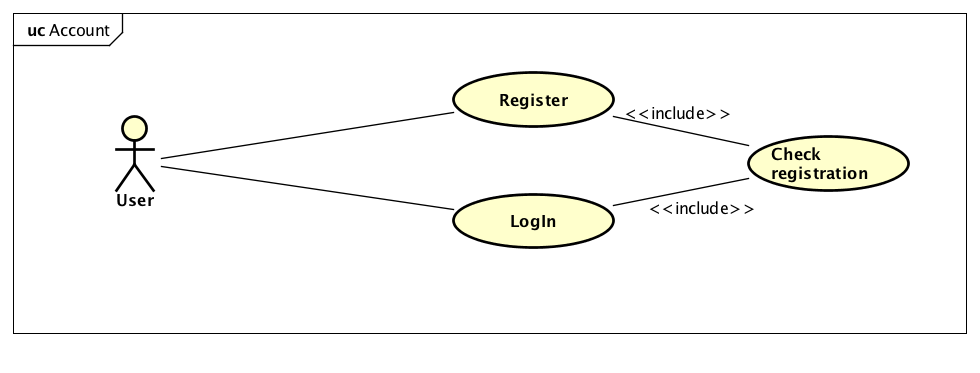
\includegraphics[width=380px]{img/usecase_login_registration}
	\caption{Use Case Login and Registration procedure. Refer to Goal 1 and 2}
\end{figure}
\FloatBarrier


